\documentclass[a4paper,12pt,titlepage]{article}
%\usepackage[T1]{fontenc}

\usepackage{titlesec}
\usepackage{titling}
\usepackage[portuguese]{babel}
\usepackage[utf8x]{inputenc}
\usepackage{indentfirst}
\usepackage{graphicx}
%\usepackage{times}
\usepackage{ucs}
\usepackage{float}    
\usepackage{fancyvrb}   
\usepackage{verbatim}
\usepackage{listings}
\usepackage{hyperref}
\usepackage{epigraph}
\usepackage{listings}
\usepackage{tabularx}
\usepackage{lipsum}

\hypersetup{
    colorlinks=true,       
    linkcolor=black,          
    citecolor=black,   
    filecolor=black,  
    urlcolor=black  
}

\hyphenation {di-re-cio-na-men-to} 

%\renewcommand*{\familydefault}{\ttdefault}
\lstset{columns=fullflexible,basicstyle=\ttfamily}

\title{\large
Universidade Federal de Minas Gerais \\ \
Instituto de Ciências Exatas \\ \ 
Departamento de Ciência da Computação \\ \
\\[1cm]
Projeto e Análise de Algoritmos\\ \
3º Trabalho Prático - Paradigmas de Programação\\ \
\\[1cm]
\textbf{\Large A Spy History}
\\[1cm]
}

\author{\large Alberto Hideki Ueda \\[0.5cm] 
	Orientador: Berthier Ribeiro Neto 
\\[3cm] }

\date{\textsc{Belo Horizonte\\ \
14 de novembro de 2014}}

\begin{document}
\maketitle

\pagebreak

\section{Descrição do problema}

Dada um mensagem composta de \textit{bits} `0' e `1' e possíveis erros de transmissão, representados pelo símbolo `-', determinar se existe ou não um comando de controle na mensagem. Um erro de transmissão pode ser tanto um `0' quanto um `1'. Um comando de controle ou é uma sequência ``000" ou uma sequência ``11111". A resposta deve ser uma das seguintes:

\[
Resposta = 
\left \{
\begin{tabular}{lll}
$true$, se a mensagem com certeza contém um comando \\ de controle; \\
\\ 
$false$, se a mensagem com certeza não contém um \\ comando; \\
\\
$both$, se a mensagem pode ou não conter um comando,\\ dependendo do que os erros significarem. 
\end{tabular}
\right.
\]

\section{Modelagem}
% The description of the problem, how did you model it and how your algorithms work. The explanation of the algorithms must be clear, you can use pseudo-code for this.
A modelagem do problema é simples. Dada uma sequência de caracteres do conjunto $\{0, 1, -\}$ com tamanho máximo de 100 caracteres, determinar se tal sequência contém a subsequência ``000'' ou ``11111''; ou então se é possível substituir os caracteres `-' da sequência por \textit{bits} `0' e `1'  de forma que exista alguma destas subsequências. 

Há o caso particular em que mesmo que uma mensagem possua um ou mais caracteres `-', todas as formas de substituição possíveis contém subsequências de controle. Por exemplo, na mensagem ``1111-00'' todas as possíveis mensagens originais (``1111100'' e ``1111000'') contém um comando de controle. Neste e nos demais casos em que este cenário se aplica, naturalmente a resposta do algoritmo deve ser $true$.

Se há pelo menos uma possibilidade da mensagem não conter tais subsequências \textbf{E} pelo uma possibilidade dela conter, a resposta deve ser $both$.

Caso não haja nenhuma possibilidade da cadeia de caracteres conter um comando de controle, a resposta deve ser $false$. \ \\

A seguir serão descritos os três algoritmos propostos para lidar com o problema, cada um seguindo um paradigma de programação diferente.

\section{Algoritmo de Força Bruta}


\subsection{Complexidade de Espaço}
\subsection{Complexidade de Tempo}
\subsection{Análise Experimental}

\section{Algoritmo Guloso}

\subsection{Complexidade de Espaço}
\subsection{Complexidade de Tempo}
\subsection{Análise Experimental}


\section{Algoritmo com Programação Dinâmica}

\subsection{Complexidade de Espaço}
\subsection{Complexidade de Tempo}
\subsection{Análise Experimental}


\section{Dificuldades Encontradas}

\begin{figure}[H]
     \centering
     % 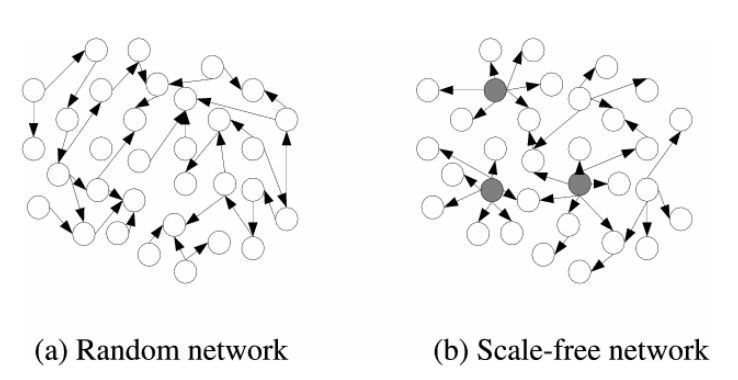
\includegraphics[scale=0.5]{figures/network-types.png}
     \caption{}
     \label{bsp}
\end{figure}

\section{Conclusão}
% A brief conclusion of the work


% Referências
\bibliographystyle{plain}%amsalpha
\bibliography{bibliografia}
\newpage

\end{document}


